% This is "sig-alternate.tex" V2.1 April 2013
% This file should be compiled with V2.5 of "sig-alternate.cls" May 2012
%
% This example file demonstrates the use of the 'sig-alternate.cls'
% V2.5 LaTeX2e document class file. It is for those submitting
% articles to ACM Conference Proceedings WHO DO NOT WISH TO
% STRICTLY ADHERE TO THE SIGS (PUBS-BOARD-ENDORSED) STYLE.
% The 'sig-alternate.cls' file will produce a similar-looking,
% albeit, 'tighter' paper resulting in, invariably, fewer pages.
%
% ----------------------------------------------------------------------------------------------------------------
% This .tex file (and associated .cls V2.5) produces:
%       1) The Permission Statement
%       2) The Conference (location) Info information
%       3) The Copyright Line with ACM data
%       4) NO page numbers
%
% as against the acm_proc_article-sp.cls file which
% DOES NOT produce 1) thru' 3) above.
%
% Using 'sig-alternate.cls' you have control, however, from within
% the source .tex file, over both the CopyrightYear
% (defaulted to 200X) and the ACM Copyright Data
% (defaulted to X-XXXXX-XX-X/XX/XX).
% e.g.
% \CopyrightYear{2007} will cause 2007 to appear in the copyright line.
% \crdata{0-12345-67-8/90/12} will cause 0-12345-67-8/90/12 to appear in the copyright line.
%
% ---------------------------------------------------------------------------------------------------------------
% This .tex source is an example which *does* use
% the .bib file (from which the .bbl file % is produced).
% REMEMBER HOWEVER: After having produced the .bbl file,
% and prior to final submission, you *NEED* to 'insert'
% your .bbl file into your source .tex file so as to provide
% ONE 'self-contained' source file.
%
% ================= IF YOU HAVE QUESTIONS =======================
% Questions regarding the SIGS styles, SIGS policies and
% procedures, Conferences etc. should be sent to
% Adrienne Griscti (griscti@acm.org)
%
% Technical questions _only_ to
% Gerald Murray (murray@hq.acm.org)
% ===============================================================
%
% For tracking purposes - this is V2.0 - May 2012

\documentclass{sig-alternate-05-2015}

\usepackage{url}                  % format URLs
\usepackage{listings}          % format code
\lstset{
  mathescape, 
  language={C},
  basicstyle=\small
}
\usepackage{enumitem}      % adjust spacing in enums
\usepackage[colorlinks=true,allcolors=blue,breaklinks,draft=false]{hyperref}   
\usepackage{graphicx}
\usepackage{float,subfig}
\usepackage{xspace,framed}
\usepackage{colortbl}
\usepackage{calc}

\usepackage{algorithm}
\usepackage{amsfonts}
\usepackage{amsmath}
\usepackage{multicol}
\usepackage{multirow}
\usepackage{tikz}
\usetikzlibrary{positioning, automata, shapes.arrows, calc, shapes, arrows}
\usepackage[justification=centering]{caption}
\usepackage{stmaryrd}
\usepackage{hhline}
\usepackage{pifont}
%\usepackage{cite}
\usepackage{pdflscape} % Experiments table is landscape
\usepackage{longtable}
\usepackage{afterpage}
\usepackage{wasysym}


\begin{document}

% Copyright
\setcopyright{acmcopyright}
%\setcopyright{acmlicensed}
%\setcopyright{rightsretained}
%\setcopyright{usgov}
%\setcopyright{usgovmixed}
%\setcopyright{cagov}
%\setcopyright{cagovmixed}


% DOI
\doi{}

% ISBN
\isbn{}

%Conference
%\conferenceinfo{PLDI '13}{June 16--19, 2013, Seattle, WA, USA}

%\acmPrice{\$15.00}

%
% --- Author Metadata here ---
%\conferenceinfo{WOODSTOCK}{'97 El Paso, Texas USA}
%\CopyrightYear{2007} % Allows default copyright year (20XX) to be over-ridden - IF NEED BE.
%\crdata{0-12345-67-8/90/01}  % Allows default copyright data (0-89791-88-6/97/05) to be over-ridden - IF NEED BE.
% --- End of Author Metadata ---

\title{TBD}
%\subtitle{[Extended Abstract]
%\titlenote{A full version of this paper is available as
%\textit{Author's Guide to Preparing ACM SIG Proceedings Using
%\LaTeX$2_\epsilon$\ and BibTeX} at
%\texttt{www.acm.org/eaddress.htm}}}
%
% You need the command \numberofauthors to handle the 'placement
% and alignment' of the authors beneath the title.
%
% For aesthetic reasons, we recommend 'three authors at a time'
% i.e. three 'name/affiliation blocks' be placed beneath the title.
%
% NOTE: You are NOT restricted in how many 'rows' of
% "name/affiliations" may appear. We just ask that you restrict
% the number of 'columns' to three.
%
% Because of the available 'opening page real-estate'
% we ask you to refrain from putting more than six authors
% (two rows with three columns) beneath the article title.
% More than six makes the first-page appear very cluttered indeed.
%
% Use the \alignauthor commands to handle the names
% and affiliations for an 'aesthetic maximum' of six authors.
% Add names, affiliations, addresses for
% the seventh etc. author(s) as the argument for the
% \additionalauthors command.
% These 'additional authors' will be output/set for you
% without further effort on your part as the last section in
% the body of your article BEFORE References or any Appendices.

%\numberofauthors{8} %  in this sample file, there are a *total*
% of EIGHT authors. SIX appear on the 'first-page' (for formatting
% reasons) and the remaining two appear in the \additionalauthors section.
%
%% \author{
%% % You can go ahead and credit any number of authors here,
%% % e.g. one 'row of three' or two rows (consisting of one row of three
%% % and a second row of one, two or three).
%% %
%% % The command \alignauthor (no curly braces needed) should
%% % precede each author name, affiliation/snail-mail address and
%% % e-mail address. Additionally, tag each line of
%% % affiliation/address with \affaddr, and tag the
%% % e-mail address with \email.
%% %
%% % 1st. author
%% \alignauthor
%% Ben Trovato\titlenote{Dr.~Trovato insisted his name be first.}\\
%%        \affaddr{Institute for Clarity in Documentation}\\
%%        \affaddr{1932 Wallamaloo Lane}\\
%%        \affaddr{Wallamaloo, New Zealand}\\
%%        \email{trovato@corporation.com}
%% % 2nd. author
%% \alignauthor
%% G.K.M. Tobin\titlenote{The secretary disavows
%% any knowledge of this author's actions.}\\
%%        \affaddr{Institute for Clarity in Documentation}\\
%%        \affaddr{P.O. Box 1212}\\
%%        \affaddr{Dublin, Ohio 43017-6221}\\
%%        \email{webmaster@marysville-ohio.com}
%% }

\maketitle
\begin{abstract}

\end{abstract}


%
% The code below should be generated by the tool at
% http://dl.acm.org/ccs.cfm
% Please copy and paste the code instead of the example below. 
%
%% \begin{CCSXML}
%% <ccs2012>
%%  <concept>
%%   <concept_id>10010520.10010553.10010562</concept_id>
%%   <concept_desc>Computer systems organization~Embedded systems</concept_desc>
%%   <concept_significance>500</concept_significance>
%%  </concept>
%%  <concept>
%%   <concept_id>10010520.10010575.10010755</concept_id>
%%   <concept_desc>Computer systems organization~Redundancy</concept_desc>
%%   <concept_significance>300</concept_significance>
%%  </concept>
%%  <concept>
%%   <concept_id>10010520.10010553.10010554</concept_id>
%%   <concept_desc>Computer systems organization~Robotics</concept_desc>
%%   <concept_significance>100</concept_significance>
%%  </concept>
%%  <concept>
%%   <concept_id>10003033.10003083.10003095</concept_id>
%%   <concept_desc>Networks~Network reliability</concept_desc>
%%   <concept_significance>100</concept_significance>
%%  </concept>
%% </ccs2012>  
%% \end{CCSXML}

%% \ccsdesc[500]{Computer systems organization~Embedded systems}
%% \ccsdesc[300]{Computer systems organization~Redundancy}
%% \ccsdesc{Computer systems organization~Robotics}
%% \ccsdesc[100]{Networks~Network reliability}


%
% End generated code
%

%
%  Use this command to print the description
%
\printccsdesc

% We no longer use \terms command
%\terms{Theory}

\keywords{}

\section{Introduction}

We are interested in the stability of closed-loop systems, i.e., controllers along with a
model of their physical environment, the plant, as shown in Fig.~\ref{fig:closed-system}.

\begin{figure*}
\centering
\resizebox{.5\textwidth}{!}{
 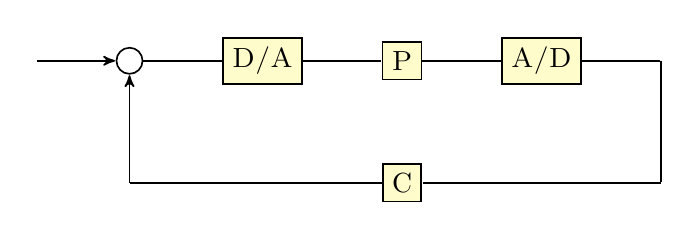
\begin{tikzpicture}[scale=0.3,-,>=stealth',shorten >=.2pt,auto,
     semithick, initial text=, ampersand replacement=\&,]

  \matrix[nodes={draw, fill=none, shape=rectangle, minimum height=.2cm, minimum width=.2cm, align=center}, row sep=1cm, column sep=1cm] {
   \coordinate (aux0);
   \& \node[circle] (circle) {}; 
   \& \node[fill=yellow!20] (da) {{\sc D/A}}; 
   \& \node[fill=yellow!20] (p) {{\sc P}};
   \& \node[fill=yellow!20] (ad) {{\sc A/D}}; 
   \& \coordinate (aux1);\\
   \& \coordinate (aux3); 
   \&
   \&
   \node[fill=yellow!20] (c) {C};
   \& 
   \& \coordinate (aux2);\\
  };


  \path[->] (aux0) edge (circle.west);
  \path  
   (circle.east) edge (da.west)
   (da.east) edge (p.west)
   (p.east) edge (ad.west)
   (ad.east) edge (aux1.west)
   (aux1.south) edge (aux2.north)
   (aux2.west) edge (c.east)
   (c.west) edge (aux3.east); 
  \path[->]  (aux3.north) edge (circle.south);
 \end{tikzpicture}
}
 \caption{Closed-Loop System. \label{fig:closed-system}}
\end{figure*}




\section{Overview}
\section{Running Example}
\section{Program Synthesis}

We use CounterExample-Guided Inductive Synthesis (CEGIS), as illustrated in Fig~\ref{fig:CEGIS}.

\begin{figure*}
\centering
\resizebox{.7\textwidth}{!}{
 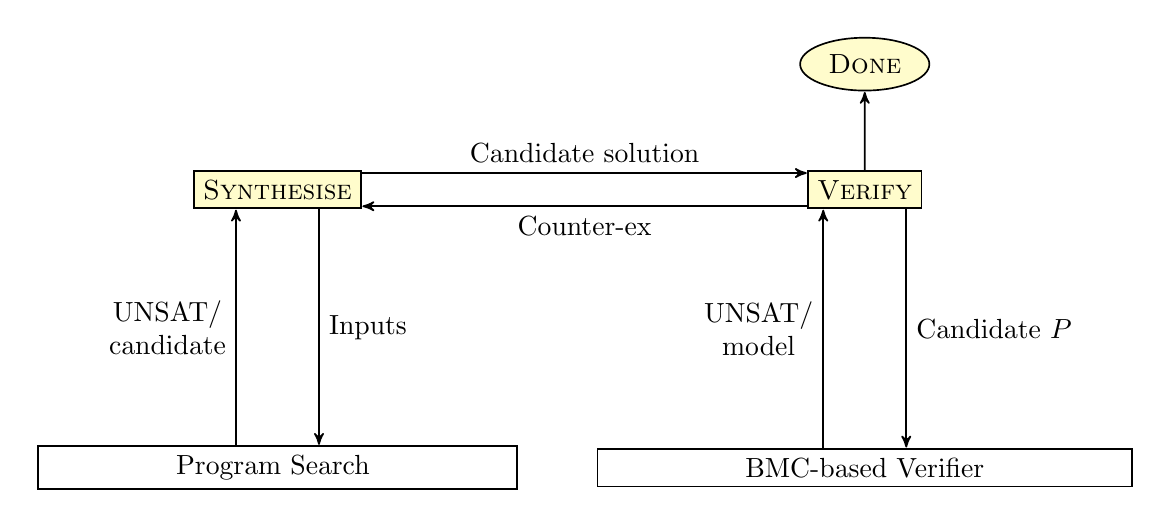
\begin{tikzpicture}[scale=0.3,->,>=stealth',shorten >=.2pt,auto, semithick, initial text=, ampersand replacement=\&,]
  \matrix[nodes={draw, fill=none, shape=rectangle, minimum height=.2cm, minimum width=.2cm, align=center
},
          row sep=1cm, column sep=1cm] {
   \& \node[ellipse, fill=yellow!20] (done) {{\sc Done}}; \\
   \node[fill=yellow!20] (synth) {{\sc Synthesise}};
   \&
   \node[fill=yellow!20] (verif) {{\sc Verify}}; \\

   \& \\
   \& \\
   \node (gp) {~~~~~~~~~~~~~~Program Search~~~~~~~~~~~~~~~};
   \&
   \node (bmc) {~~~~~~~~~~~~~~~BMC-based Verifier~~~~~~~~~~~~~~~};
   
    \\
  };

   \path
    ([yshift=2em]synth.east) edge node {Candidate solution} ([yshift=2em]verif.west)
    ([yshift=-2em]verif.west) edge node {Counter-ex} ([yshift=-2em]synth.east)
    ([xshift=5em]verif.south) edge node {Candidate $P$} ([xshift=5em]bmc.north)
    ([xshift=-5em]bmc.north) edge node[align=center]  {UNSAT/\\model} ([xshift=-5em]verif.south)
    (verif) edge node {} (done)
    ([xshift=5em]synth.south) edge node[align=center] {Inputs} ([xshift=5em]gp.north)
    ([xshift=-5em]gp.north) edge node[align=center] {UNSAT/\\candidate} ([xshift=-5em]synth.south);
 \end{tikzpicture}
}
 \caption{Counterexample-Guided Inductive Synthesis. \label{fig:CEGIS}}
\end{figure*}

\section{Experiments}
\section{Related Works}

\paragraph{Robustness analyses of closed-loop systems} The analysis in 
\cite{DBLP:conf/hybrid/WangGRJF16}
relies on an invariant computation
on the discrete system dynamics.

\paragraph{Stability analyses of closed-loop systems} 
In \cite{DBLP:conf/hybrid/RouxJG15}, the authors
perform the analysis in the state space
domain using Lyapunov-based quadratic invariants.
In \cite{DBLP:journals/corr/PakmehrWJVF13}, Pakmehr et al. 
design a control software verification framework for gas turbine engines.

\paragraph{Uses of CEGIS for control sysnthesis} 
In \cite{DBLP:conf/cdc/RavanbakhshS15}, Ravanbakhsh and Sankaranarayanan use
CEGIS for the synthesis of switching
controllers for stabilizing continuous-time plants.


\section{Conclusions}

%
% The following two commands are all you need in the
% initial runs of your .tex file to
% produce the bibliography for the citations in your paper.
\bibliographystyle{abbrv}
\bibliography{paper}  % sigproc.bib is the name of the Bibliography in this case
% You must have a proper ".bib" file
%  and remember to run:
% latex bibtex latex latex
% to resolve all references
%
% ACM needs 'a single self-contained file'!
%
%APPENDICES are optional
%\balancecolumns
%\appendix
%Appendix A
\end{document}
